\documentclass{report}
\usepackage[margin=1in, paperwidth=8.5in, paperheight=11in]{geometry}
%Math packages%
\usepackage{amsmath}
\usepackage{amsthm}
%Spacing%
\usepackage{setspace}
%Package to adjust indentation%
\usepackage{changepage}
\onehalfspacing
%Lecture number%
\newcommand{\lectureNum}{1}
%Variables - Date and Course%
\newcommand{\curDate}{February 9, 2017}
\newcommand{\course}{CS 241}
%Defining the example tag%
%\theoremstyle{definition}%
\newtheorem{ex}{Example}[section]
%Setting counter given the lecture number%
\setcounter{chapter}{\lectureNum{}}
%Package to insert code%
\usepackage{listings}
\usepackage{courier}
\usepackage{xcolor}
\lstset { 
    tabsize=2,
    breaklines=true,
    language=C++,
    backgroundcolor=\color{blue!8}, % set backgroundcolor
    basicstyle=\footnotesize\ttfamily,% basic font setting
}
%Package to draw trees%
\usepackage{tikz}
\begin{document}
%Note title%
\begin{center}
\begin{Large}
\textsc{CS 241 Midterm Review}\\
\end{Large}
Bartosz Antczak\\
\textit{These are answers to the questions outlined in the sample review questions on the CS 241 course website. In addition, not all of the questions were covered in this review section.}
\end{center} 
\subsubsection{Topics to be Covered}
\begin{enumerate}
\item Data Representation
\item MIPS Programming
\item MIPS Assembly
\item Regular Languages
\item CFL
\end{enumerate}
% Actual Notes%

\section{MIPS Programming}
Big part of the midterm.
\begin{itemize}
\item[1.] \texttt{\$1} will store the value of array \texttt{A}, and \texttt{\$2} will store the value of array \texttt{B}.
\begin{lstlisting}
lis $14
.word 4
lis $12
.word 2
multu $14, $3
mflo $21
add $22, $4, $1 ; A[$3] address
add $23, $21, $2 ; B[$3] address
lw $26, 0($22) ; A[$3] loaded into $26
lw $27, 0($23) ; B[$3] loaded into $27
mult $14, $4
mflo $21
add $24, $21, $1
add $25, $21, $2
lw $28, 0($24)
lw $29, 0($25)
slt $8, $26, $27
slt $9, $29, $28
add $10, $8, $9
bne $10, $12, 1
sw $29, 0($22) ; A[$3] = B[$4]: store the value in B[$4] in the address of A[$3]
jr $31
\end{lstlisting}
\item[3.] We'll use the Euclidean algorithm (ah, back to the MATH 135 days). Recall that the algorithm is structured as:
$$
\gcd(m,n)=
\begin{cases}
n & \mathrm{if}\, m\%n = 0\\
\gcd(n, m\%n) & \text{otherwise}\\
\end{cases}
$$
\begin{lstlisting}
gcd:
	divu $1, $2
	mfhi $3
	beq $3, $0, end
	add $1, $2, $0
	add $2, $3, $0
	sw $31, -4($30) ; save return address
	lis $31
	.word 4
	sub $30, $30, $31
	lis $4
	.word gcd
	jalr $4
	lis $31
	.word 4
	add $30, $30, $31
	lw $31, -4($30)
end:
	jr $31
\end{lstlisting}
\end{itemize}
\section{NFA's (Non-Deterministic Finite Automata)}
Recall that a NFA is a DFA, where states can have multiple transitions for the same label.
\begin{itemize}
\item[3(b).] Give a NFA over the language $L$, where $\Sigma = \{0,1,2,3\}$ that contains all strings that end with 233.
\begin{figure}[ht]
\begin{center}
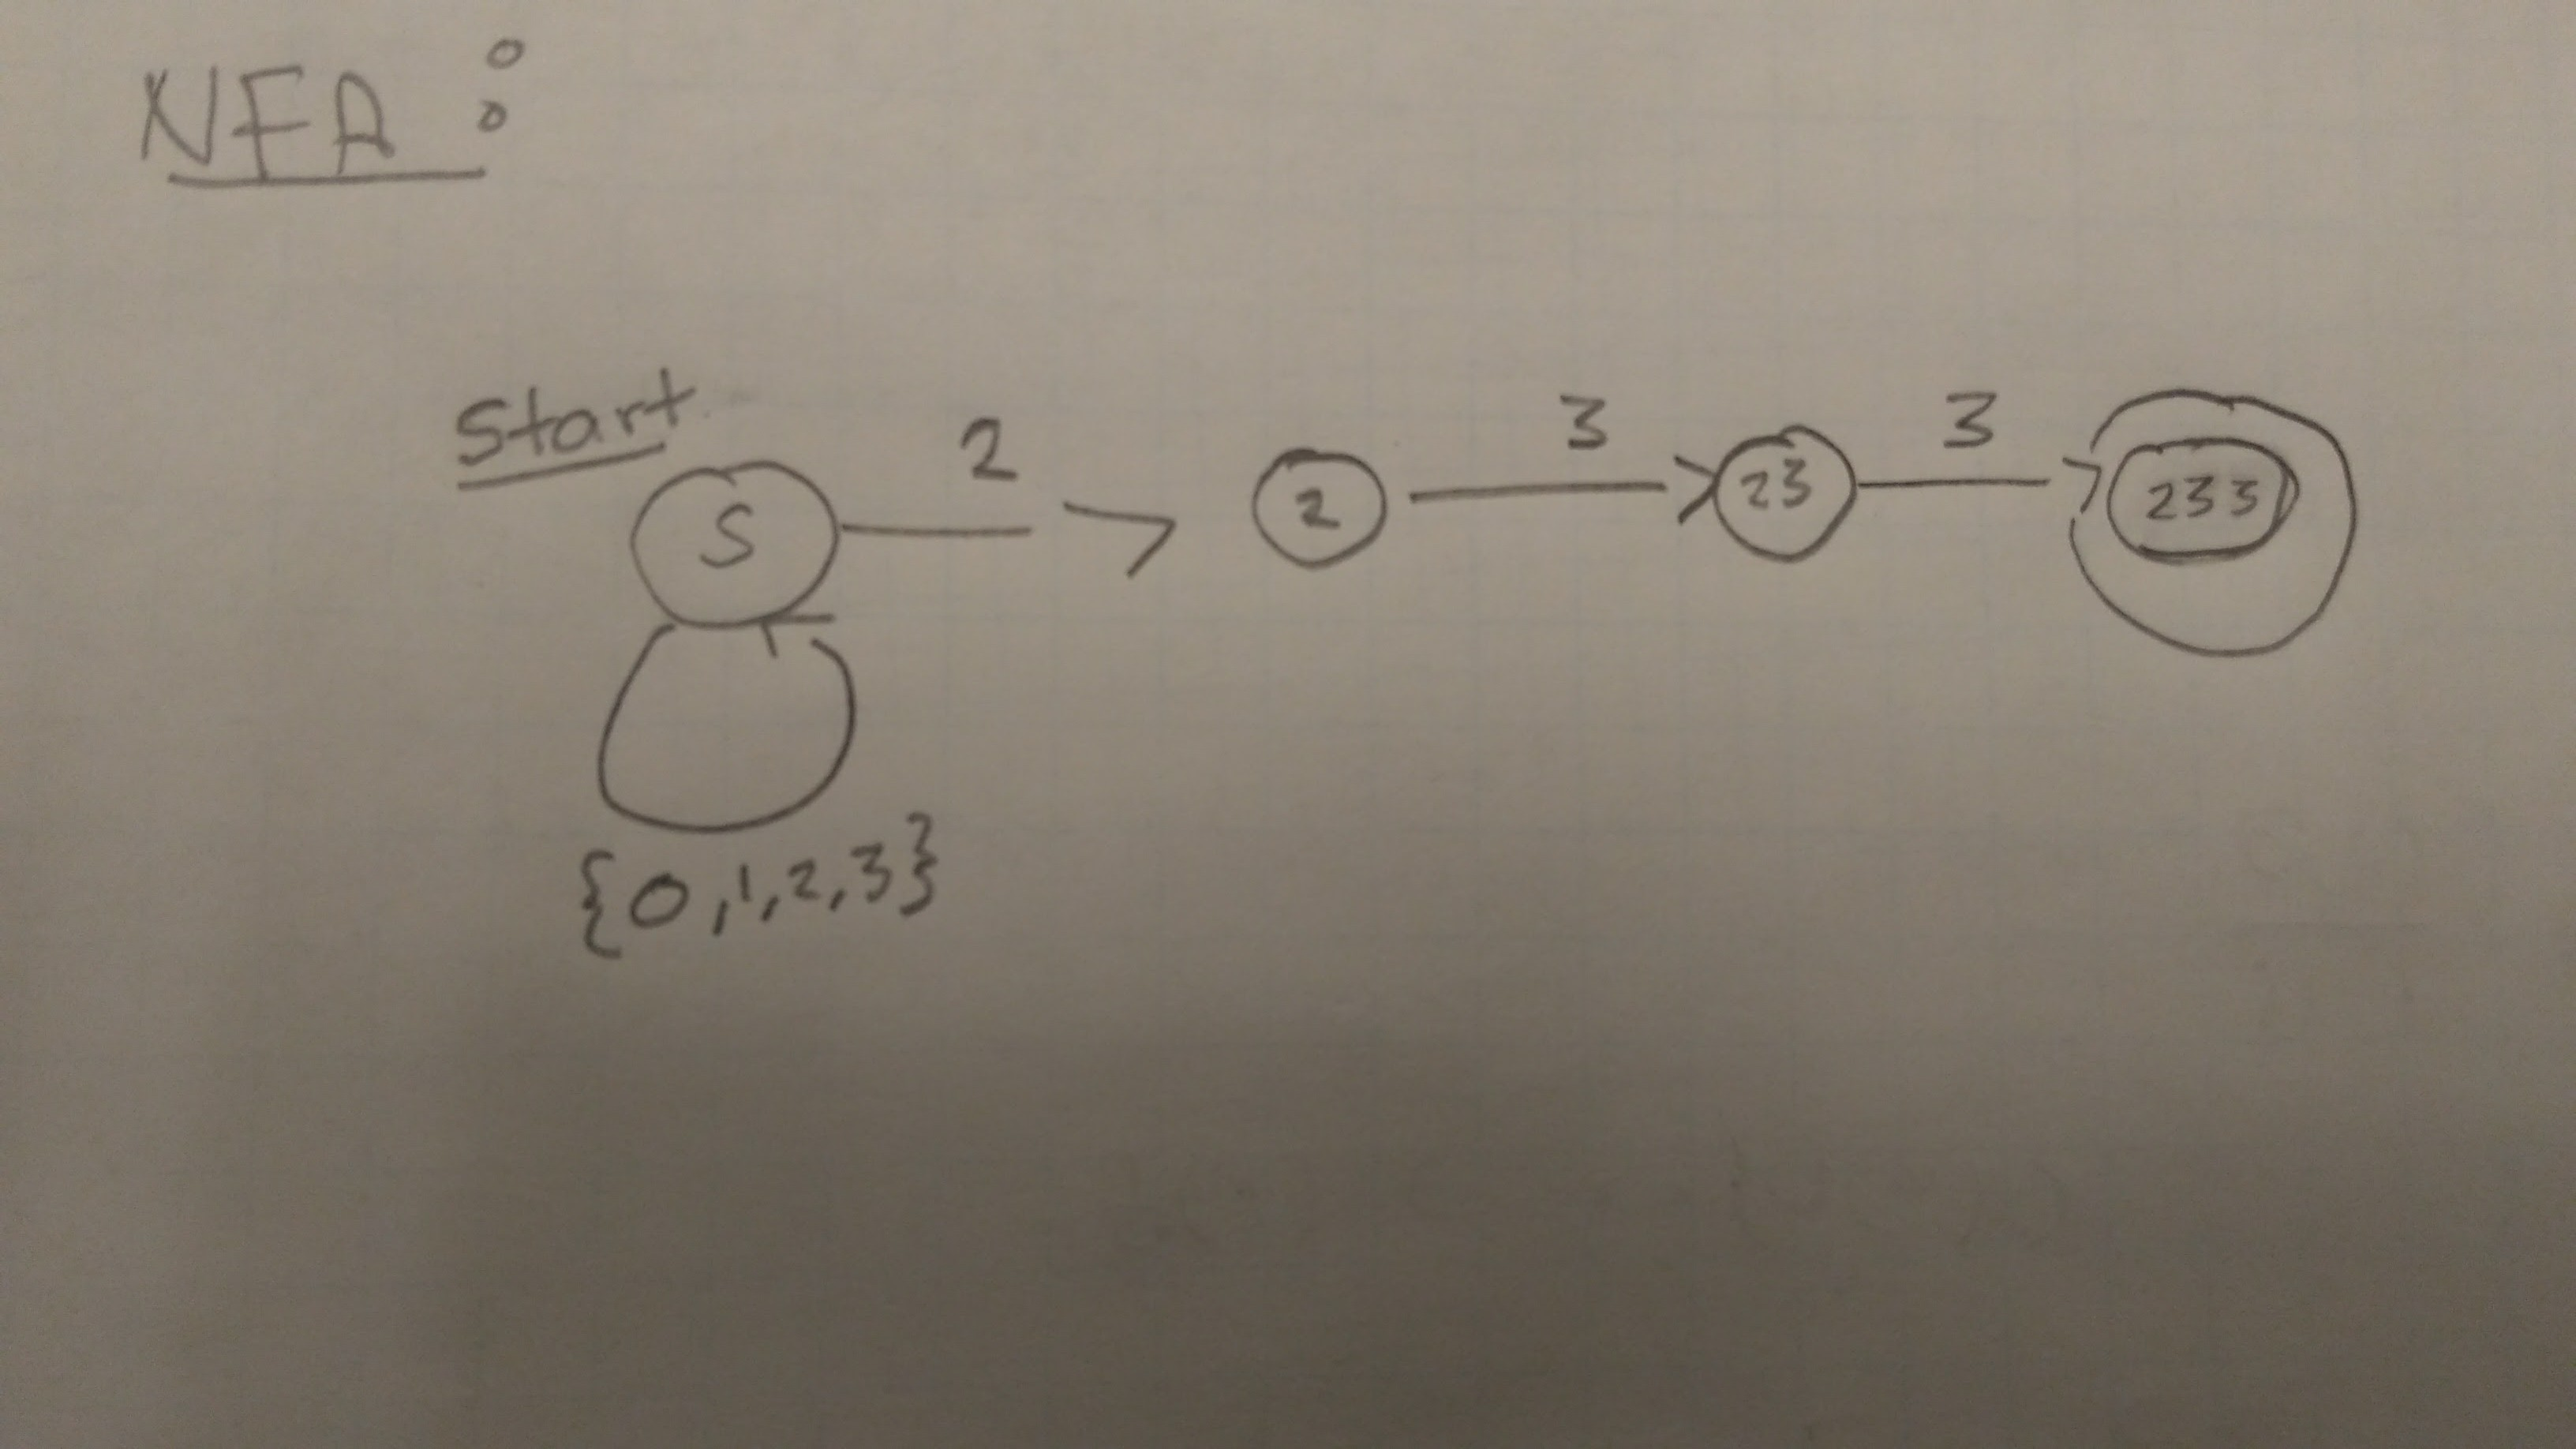
\includegraphics[scale=0.1]{nfa1.jpg}
\end{center}
\end{figure}
\item[4.] Since it's finite, we can list all of the possible sets of words for each state
\begin{center}
\begin{tabular}{ r || c | c }
& a & b \\ \hline
0 & \{0,1\} & \{0,2\} \\ 
1 & \{\} & \{2,3\} \\ 
2 & \{1,3\} & \{\} \\ 
3 & \{\} & \{\} \\ 
\end{tabular}
\end{center}
Now we look at all cases of multiple set transitions:
\begin{center}
\begin{tabular}{ r || c | c }
& a & b \\ \hline
01 & \{0,1\} & \{0,2,3\} \\ 
02 & \{0,1,3\} & \{0,2\} \\ 
23 & \{1,3\} & \{\} \\ 
13 & \{\} & \{2,3\} \\ 
023 & \{0,1,3\} & \{0,2\} \\ 
013 & \{0,1\} & \{0,2,3\} \\ 
\end{tabular}
\end{center}
Drawn out, the DFA will look like:
\begin{figure}[ht]
\begin{center}
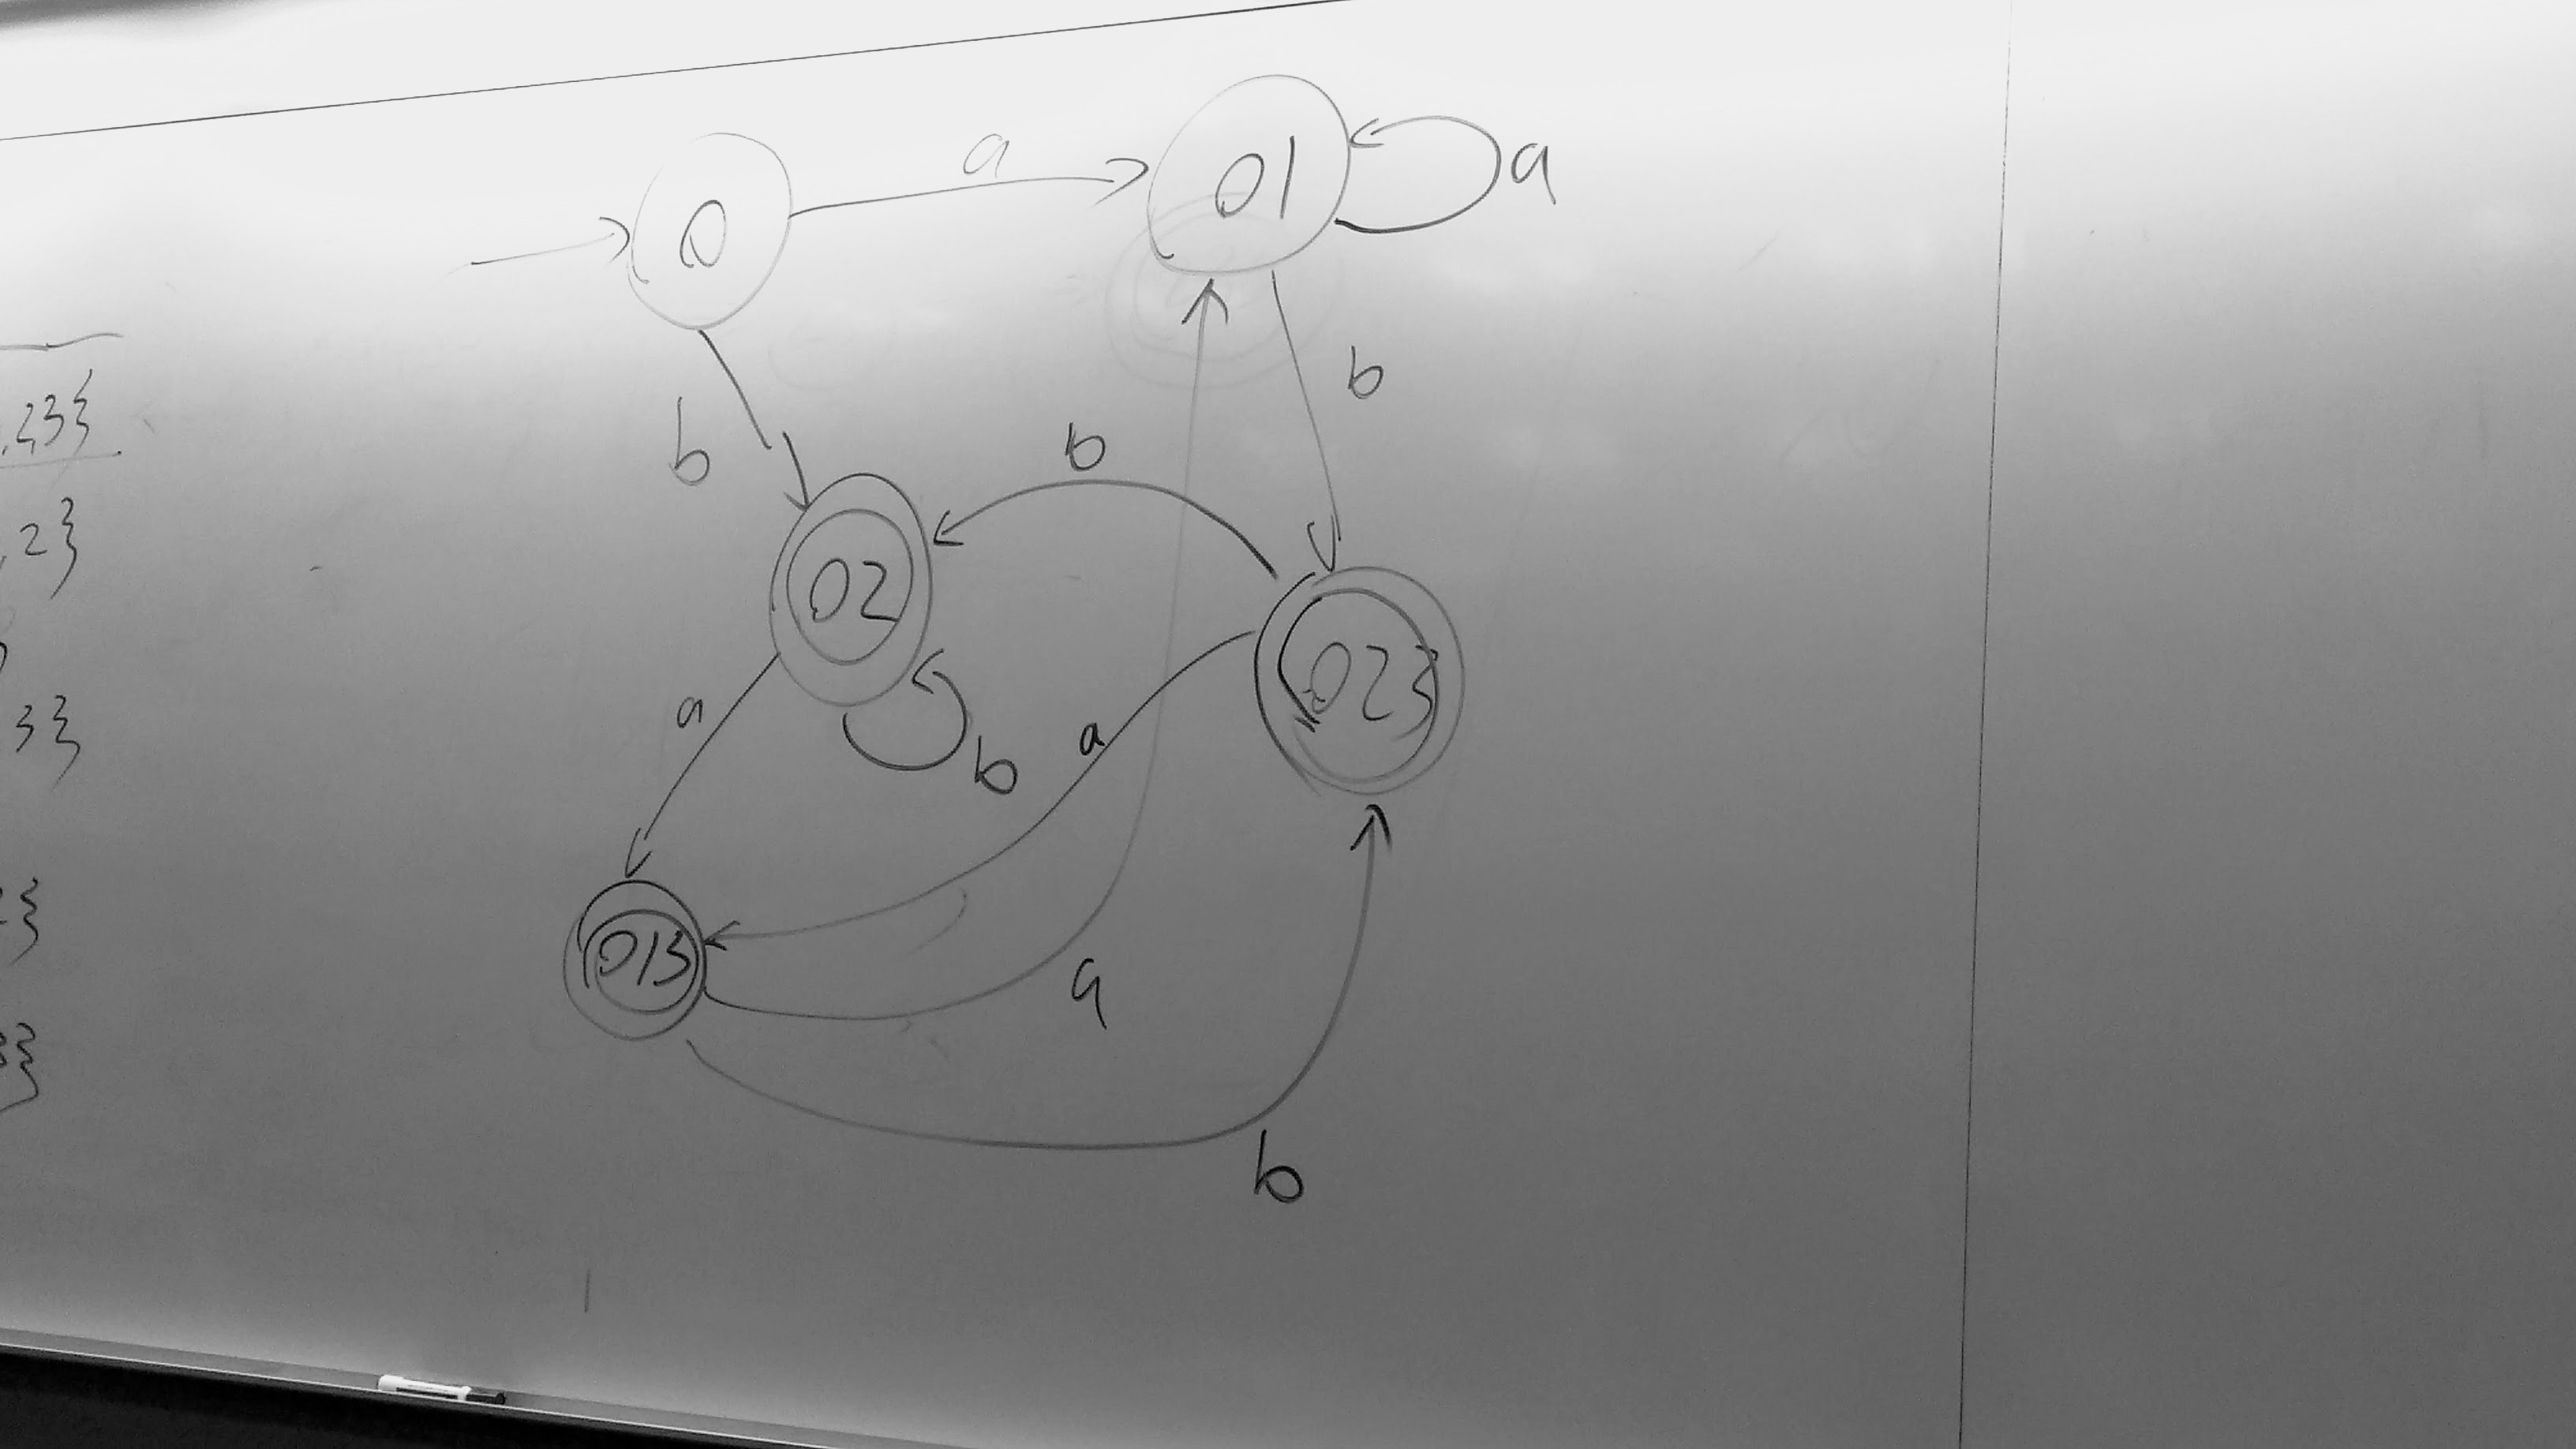
\includegraphics[scale=0.15]{dfa1.jpg}
\end{center}
\end{figure}
\end{itemize}
\section{Context-Free Languages}
\begin{itemize}
\item[3(a)] The word `aaa' is ambiguous.
\item[3(b)] An unambiguous CFG which describes the same language is:
\begin{itemize}
\item $S \rightarrow E + T$
\item $E \rightarrow E + T$
\item $E \rightarrow a$
\item $E \rightarrow T$
\end{itemize}
\end{itemize}
%END%
\end{document}
